\chapter{Design e implementazione}
\label{ch:sistema}

\section{Introduzione}
Inizieremo con una panoramica generale dell'architettura
del sistema, per poi passare a una descrizione dettagliata
dei componenti principali.

\section{Architettura del sistema}
\label{sec:architettura}
L'architettura del sistema è composta dalle seguenti componenti principali:

\begin{itemize}
      \item \textbf{Frontend}: consiste in una estensione per il browser che
            permette di interagire con il sistema.
      \item \textbf{Backend}: è il server che gestisce le richieste
            provenienti dal frontend e comunica con il database e il LLM.
      \item \textbf{Embedder}: è il componente che genera gli embedding
            delle parole chiave che popolano il database, nonchè gli embedding
            delle richieste provenienti dal frontend.
      \item \textbf{Database}: memorizza le informazioni relative agli embedding
            delle parole chiave che fungono da input al LLM.
            Fornisce inoltre, il contesto aggiuntivo utile a generare
            le risposte.
      \item \textbf{LLM}: è il modello che genera le risposte in base
            alle richieste del frontend.
\end{itemize}

\begin{figure}
      \centering
      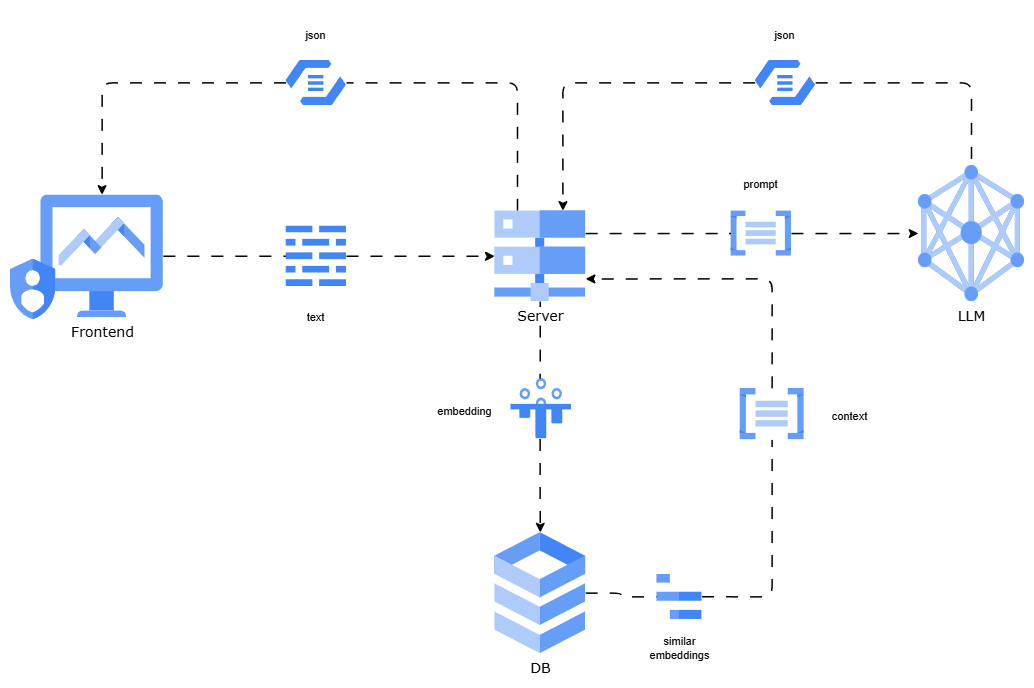
\includegraphics[width=1\textwidth]{res/architecture2.png}
      \caption{Architettura del sistema e flusso dei dati}
      \label{fig:architettura}
\end{figure}

\section{Componenti principali}
\label{sec:componenti}
\subsection{Frontend}
\label{sec:frontend}
Il frontend è un'estensione per il browser che consente di
interagire con una qualsiasi pagina web.
L'estensione è progettata per essere leggera e veloce, in
modo da non influire sulle prestazioni del browser.

Il frontend è responsabile della raccolta delle
informazioni, oltre che della visualizzazione dei
risultati.
Quando l'utente seleziona un elemento della pagina, il
frontend estrae il contenuto testuale e lo invia al backend
per l'elaborazione.
Il backend genera quindi una risposta e la invia al
frontend, che la mostra all'utente.

Inoltre, il frontend permette di selezionare quale modello
utilizzare per generare le risposte, in modo da poter
testare le prestazioni di diversi modelli.

\subsection{Backend}
\label{sec:backend}

Il backend è il cuore del sistema, responsabile della
gestione delle richieste provenienti dal frontend e della
comunicazione con il database e il LLM.
Il backend è implementato in Python e utilizza il framework
FastAPI che permette la creazione di API RESTful, per
applicazioni web scalabili e performanti.
Il backend è progettato per essere modulare e facilmente
configurabile, in modo da poter aggiungere nuove
funzionalità in futuro.

Quando il backend riceve una richiesta dal frontend, esegue
le seguenti operazioni:
\begin{itemize}
      \item Preprocessa il contenuto testuale della richiesta
      \item Tokenizza il testo dividendo il testo in frasi
            più piccole.\\
            \textbf{Questo passaggio è fondamentale per creare il contesto
                  necessario per il LLM.}
      \item Genera gli embedding di ogni frase attraverso
            l'embedder.
      \item Esegue una ricerca nel database per trovare le
            parole chiave più simili agli embedding generati
      \item Invia la richiesta al LLM per generare la risposta.
            La richiesta al LLM include il contenuto processato e le
            parole chiave trovate nel database.
      \item Restituisce la risposta del LLM al frontend sotto forma di
            JSON.
\end{itemize}

La comunicazione tra il server e il LLM avviene tramite la
libreria di OpenAI, che consente di inviare richieste al
modello e ricevere le risposte utilizzando una interfaccia
configurabile.
In particolare, la libreria permette di utilizzare qualiasi
modello compatibile con l'interfaccia di OpenAI e questo ha
permesso di testare diversi modelli attraverso il tool
\textbf{Ollama}.

\subsection{Ollama}
\label{sec:ollama}
Ollama è un tool open source che consente di eseguire LLM
localmente, senza la necessità di una connessione a
Internet.
Ollama stato è progettato per essere semplice da usare e
consente di eseguire LLM in modo rapido e efficiente
sfruttando l'accelerazione hardware delle GPU quando
possibile.
Ollama offre una varieta di modelli LLM pre-addestrati, tra
cui \textbf{Llama}\cite{touvron2023llama},
\textbf{Mistral}\cite{jiang2023mistral},
\textbf{Phi}\cite{phi-4},
\textbf{Deepseek}\cite{deepseek-ai2025deepseekr1} e
\textbf{Gemma}\cite{gemma_2025}.

In particolare, \textbf{Gemma} è il modello utilizzato per
testare il sistema, in quanto è ottimizzato per l'uso in
locale e offre prestazioni eccellenti rispetto a modelli di
dimensioni comparabili\cite{gemma_2025}.

\subsection{Embedder}
\label{sec:embedder}
L'embedder è il componente responsabile della generazione
degli embedding delle parole chiave che popolano il
database, nonchè degli embedding delle richieste del
frontend.
L'embedder è implementato in Python e utilizza la libreria
\texttt{SentenceTransformers}\cite{reimers-2019-sentence-bert}
per generare gli embedding delle parole chiave e delle
richieste.

Attraverso l'uso di \texttt{SentenceTransformers} è stato
possibile eseguire il fine-tuning del modello di embedding
\texttt{all-MiniLM-L6-v2} per ottimizzare le prestazioni
del sistema.
Il fine-tuning del modello è stato eseguito utilizzando un
dataset autonomamente creato, tramite l'uso di un web
scraper che ha estratto le informazioni da fonti pubbliche
disponibili su Internet.

Il dataset è composto da una serie di articoli e documenti
che sono stati manipolati per estrarre il contenuto
testuale e le parole chiave.

\section{Dataset e tool utilizzati}
\label{sec:dataset}

Qui di seguito sono riportati i tool e le librerie
utilizzati per la creazione del dataset e il fine-tuning
del modello di embedding:

\begin{itemize}
      \item \textbf{Puppeteer}: è una libreria Node.js che consente di
            controllare un browser Chrome o Chromium in modo
            programmatico.
      \item \textbf{Pandas}: è una libreria Python per la manipolazione e
            l'analisi dei dati.
      \item \textbf{Visualizer}: un tool creato appositamente per
            visualizzare i risultati dello scraping, utilizzato per
            verificare la correttezza dei dati estratti e studiare le
            relazioni tra le parole chiave e i documenti.
\end{itemize}

\begin{figure}[H]
      \centering
      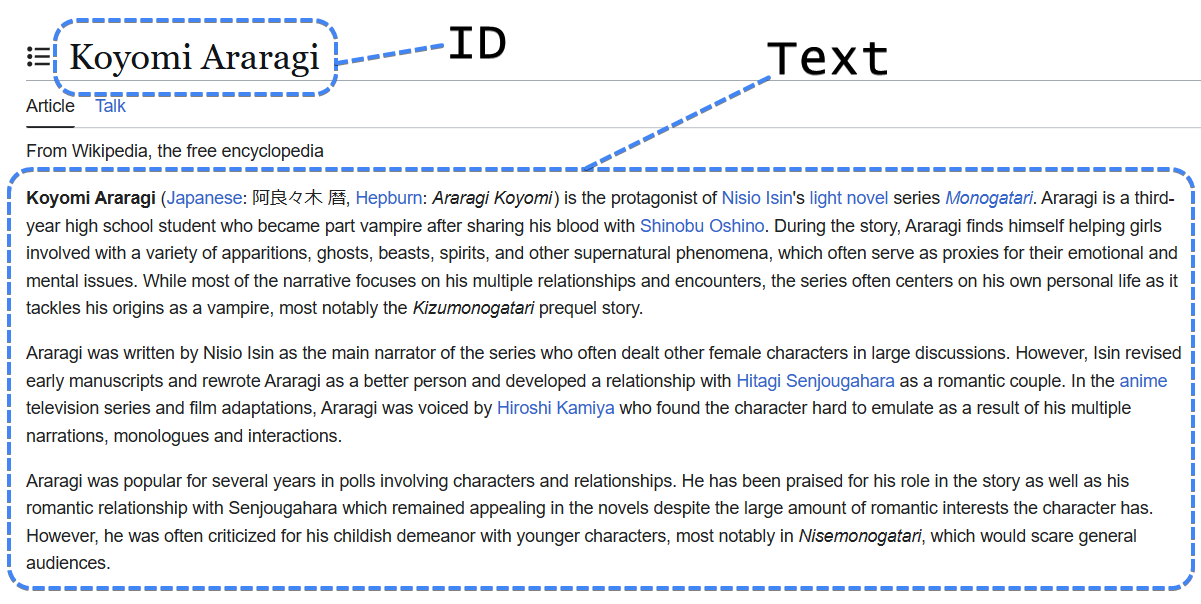
\includegraphics[width=0.8\textwidth]{res/scraper.png}
      \caption{Esempio di scraping. Fonte: Wikipedia}
      \label{fig:visualizer}
\end{figure}

In figura \ref{fig:visualizer} è mostrato un esempio di
scraping effettuato attraverso il tool, che ha estratto il
contenuto testuale di una pagina Wikipedia.

Notiamo che il tool è in grado di estrarre non solo il
contenuto testuale, ma anche i collegamenti ad altre pagine
presenti nei singoli paragrafi, unitamente a una serie di
metadati.
Ciò ha reso possibile la creazione di un grafo delle
relazioni tra le parole chiave e i documenti, che è stato
utilizzato per il fine-tuning del modello di embedding.
Il grafo è stato creato utilizzando la libreria
\texttt{D3.js}, che consente di creare visualizzazioni
interattive dei dati.

\subsection{Visualizer}
\label{sec:visualizer}
Il visualizer è stato creato appositamente per studiare le
relazioni tra le parole chiave e i documenti, in modo da
ottimizzare il fine-tuning del modello di embedding creando
un dataset bilanciato e di qualità superiore.

\begin{figure}[H]
      \centering
      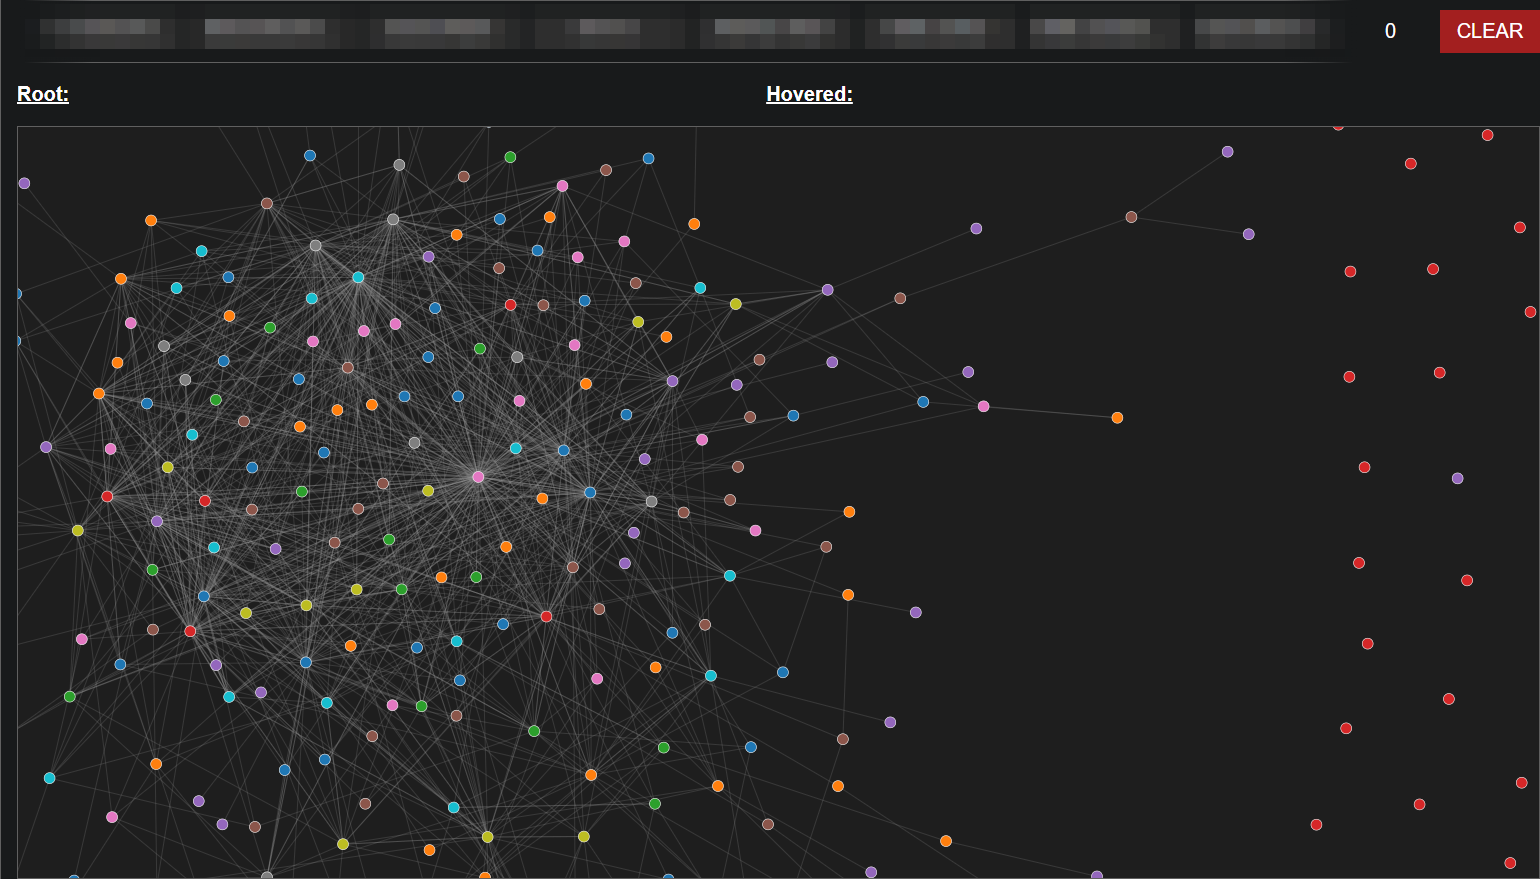
\includegraphics[width=0.8\textwidth]{res/vis1.png}
      \caption{Esempio di grafo creato dal visualizer}
      \label{fig:vis1}
\end{figure}

In figura \ref{fig:vis1} è mostrato un esempio di grafo.
Ogni nodo rappresenta un documento e ogni arco rappresenta
una relazione tra due documenti.

Possiamo osservare che alcuni documenti sono più connessi
di altri, il che indica che hanno diversi collegamenti, o
che diversi documenti fanno riferimento a loro.
E' anche possibile osservare che alcuni documenti sono
isolati, il che indica che non hanno collegamenti con altri
documenti.

Attraverso il visualizer è stato possibile filtrare i
documenti in base a diversi criteri, come ad esempio il
numero di collegamenti, metadati, o altri tipi di filtro.

Nella scelta dei documenti da includere nel dataset si è tenuto
conto di diversi fattori statistici \cite{Newman2010}
\cite{Newman2002Assortative} \cite{Newman2003Mixing},
elencati di seguito:

\begin{table}[htbp]
      \centering
      \begin{tabularx}{\textwidth}{@{}l @{\extracolsep{\fill}} r@{}}
            \toprule
            Statistica                           & Valore  \\
            \midrule
            Coefficiente di assortatività        & -0.4677 \\
            Mescolanza di assortatività discreta & -0.0059 \\
            Diametro del grafo                   & 9       \\
            Densità del grafo                    & 0.024   \\
            Lunghezza media del percorso         & 3.85    \\
            Nodi isolati                         & 76      \\
            \bottomrule
      \end{tabularx}
      \caption{Statistiche globali del grafo.
            Per la descrizione delle metriche, si veda la Sezione
            \ref{sec:graph_metrics}.
      }
      \label{tab:graph_stats}
\end{table}

\begin{table}[H]
      \centering
      \begin{tabularx}{\textwidth}{@{}l @{\extracolsep{\fill}} r@{}}
            \toprule
            Statistica                 & Valore \\
            \midrule
            Coefficiente di Clustering & 0.333  \\
            Componenti nel Cluster     & 258    \\
            Centralità di Closeness    & 0.365  \\
            \bottomrule
      \end{tabularx}
      \caption{Statistiche per singoli nodi.
            Per la descrizione delle metriche, si veda la Sezione
            \ref{sec:graph_metrics}.
      }
      \label{tab:node_stats}
\end{table}

\noindent
\textbf{Nota:}
I valori riportati nelle tabelle \ref{tab:graph_stats} e
\ref{tab:node_stats} sono stati generati su un dataset di
esempio per illustrare le funzionalità del visualizer.

\subsubsection{Metriche del grafo}
\label{sec:graph_metrics}
Le seguenti metriche sono state utilizzate per valutare le caratteristiche del grafo:

\begin{itemize}
      \item \textbf{Coefficiente di assortatività}: Misura la tendenza dei nodi a connettersi con altri nodi simili.
            Un valore negativo indica che i nodi tendono a connettersi
            con nodi dissimili.
      \item \textbf{Mescolanza di assortatività discreta}: Variazione del coefficiente di assortatività per attributi discreti dei nodi.
      \item \textbf{Diametro del grafo}: La massima distanza tra due nodi qualsiasi nel grafo.
      \item \textbf{Densità del grafo}: Rapporto tra il numero di archi presenti e il numero massimo possibile di archi.
      \item \textbf{Lunghezza media del percorso}: La distanza media tra tutte le coppie di nodi nel grafo.
      \item \textbf{Nodi isolati}: Numero di nodi che non sono connessi ad altri nodi.
      \item \textbf{Coefficiente di Clustering}: Misura quanto i vicini di un nodo sono connessi tra loro.
      \item \textbf{Componenti nel Cluster}: Numero di sottografi connessi nel grafo.
      \item \textbf{Centralità di Closeness}: Misura quanto un nodo è vicino a tutti gli altri nodi nel grafo.
\end{itemize}

\section{Preparazione del dataset}
\label{sec:dataset_prep}
Per preparare il dataset è stato necessario eseguire
diverse operazioni di post-processing sui dati estratti
dallo scraping.

In particolare, sono stati eseguiti i seguenti passaggi:
\begin{itemize}
      \item Rimozione dei metadati
      \item Normalizzazione del testo
      \item Oversampling di alcune parole chiave
      \item Introduzione di rumore nel dataset
      \item altre operazioni (disponibili nel codice sorgente\cite{af64_spoiler_filter})
\end{itemize}

Si è deciso di eseguire l'oversampling di alcuni tipi di
parole chiave, in modo da bilanciare il dataset e ottenere
un modello di embedding più robusto.

Un esempio di oversampling è mostrato in figura
\ref{fig:oversampling}.

\begin{figure}[H]
      \centering
      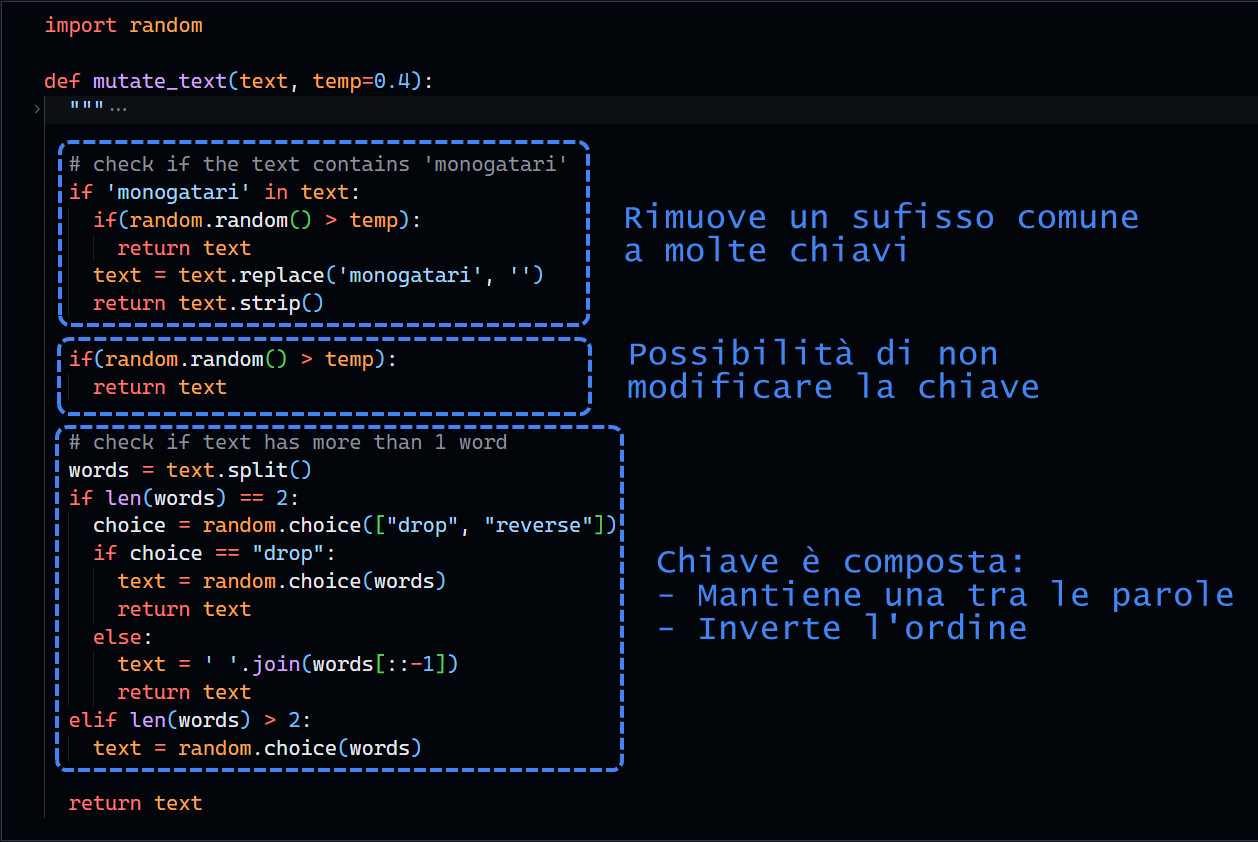
\includegraphics[width=0.7\textwidth]{res/noise.png}
      \caption{Esempio di oversampling}
      \label{fig:oversampling}
\end{figure}

Il risultato finale del dataset è stato un file JSON con il seguente formato:

\begin{table}[H]
      \centering
      \begin{tabularx}{\textwidth}{l@{\extracolsep{\fill}} l @{\extracolsep{\fill}}l}
            \toprule
            anchor         & positive                                                                                            & negative     \\
            \midrule
            koyomi araragi & vampiro, studente, adolescente                                                                      & nobile       \\
            oshino shinobu & vampiro, 500 anni, nobile                                                                           & studente     \\
            ononoki        & sissi, yay. peace peace! \faHandPeace[regular]\faEye[regular]\_\faEye[regular]\faHandPeace[regular] & hatsune miku \\
            bakemonogatari & anime, manga, light novel                                                                           & bad          \\
            \bottomrule
      \end{tabularx}
      \caption{Formato del dataset}
      \label{tab:dataset_format}
\end{table}

\noindent
\textbf{Nota:}
I dati riportati nella tabella \ref{tab:dataset_format}
sono stati generati su un dataset di esempio per illustrare
il formato del dataset.
\newline

In particolare, la colonna \texttt{anchor} contiene la
parola chiave, la colonna \texttt{positive} contiene il
contesto che si desidera associare all'ancora, mentre la
colonna \texttt{negative} contiene l'elemento che si
desidera evitare di associare alla parola chiave.

Tramite l'uso di questo formato è stato possibile separare
efficacemente le parole chiave e i contesti, in modo da
ottenere un dataset qualitativamente migliore.

\subsection{Scelta dei negativi}
\label{sec:negatives}
La scelta degli esempi negativi è stata cruciale per il
fine-tuning del modello di embedding.

Esistono principalmente due approcci per la scelta degli
esempi negativi:

\begin{itemize}
      \item \textbf{Scelta casuale}: consiste nel selezionare
            casualmente gli esempi negativi dal dataset.
      \item \textbf{Scelta non casuale}: consiste nel
            selezionare gli esempi negativi in base a regole
            stabilite.
\end{itemize}

Nel primo approccio, la scelta degli esempi negativi è
completamente casuale e non tiene conto delle relazioni tra
le parole chiave e i contesti.
Questo approccio può portare a risultati non ottimali, in
quanto gli esempi negativi potrebbero non essere
rappresentativi del contesto in cui si desidera utilizzare
il modello di embedding.

La strategia adottata nel progetto è stata quella di
estrarre randomicamente il contesto a partire dalle parole
chiave ``vicine" all'ancora di riferimento.
Questo approccio tiene conto delle relazioni tra i diversi
documenti in modo da ottenere degli embedding più robusti e
rappresentativi.

Nel nostro caso, a partire da un nodo del grafo, l'ancora è
rappresentata dal titolo del nodo, l'esempio positivo è
rappresentato dal contenuto del nodo, mentre l'esempio
negativo è rappresentato dal contenuto di un nodo
adiacente.

Questo approccio ha portato a risultati migliori rispetto
all'approccio casuale poichè sfrutta il fatto che i
documenti che hanno collegamenti in comune, molto
probabilmente condividono informazioni simili.
Permettendo al modello di distinguere tra i due, è stato
possibile ottenere un embedding più robusto e
rappresentativo.

\section{Fine-tuning del modello}
\label{sec:fine_tuning}
Il fine-tuning del modello di embedding è stato eseguito
utilizzando la libreria \texttt{SentenceTransformers} e il
dataset creato in precedenza su molteplici modelli, tra cui
\texttt{all-MiniLM-L6-v2}, per un numero di epoche pari a
4.

La \textit{loss function} utilizzata è stata la
\texttt{TripletLoss}\cite{hermans2017defense}, comunemente
utilizzata per l'addestramento di modelli di embedding.
La \texttt{TripletLoss} è progettata per minimizzare la
distanza tra l'ancora e l'esempio positivo, e massimizzare
la distanza tra l'ancora e l'esempio negativo.

Come discuteremo nel prossimo capitolo, il fine-tuning del
modello ha permesso di migliorare il modello di embedding
rendendolo più adatto al dominio in questione.
